\documentclass[submit]{harvardml}

\course{CS181-S21}
\assignment{Assignment \#2}
\duedate{7:59pm EST, Feb 19th, 2021}

\usepackage[OT1]{fontenc}
\usepackage[colorlinks,citecolor=blue,urlcolor=blue]{hyperref}
\usepackage[pdftex]{graphicx}
\usepackage{subfig}
\usepackage{fullpage}
\usepackage{amsmath}
\usepackage{amssymb}
\usepackage{framed}
\usepackage{color}
\usepackage{soul}
\usepackage{todonotes}
\usepackage{listings}
\usepackage{common}
\usepackage{enumitem}
\usepackage{bm}
\usepackage{physics}
\newcommand{\B}{\text{B}}
\newcommand{\Beta}{\text{Beta}}

\usepackage[mmddyyyy,hhmmss]{datetime}

\definecolor{verbgray}{gray}{0.9}

\lstnewenvironment{csv}{%
  \lstset{backgroundcolor=\color{verbgray},
  frame=single,
  framerule=0pt,
  basicstyle=\ttfamily,
  columns=fullflexible}}{}

\begin{document}

\begin{center}
{\Large Homework 2: Classification and Bias-Variance Trade-offs}\\
\end{center}

\subsection*{Introduction}

This homework is about classification and bias-variance trade-offs. In
lecture we have primarily focused on binary classifiers trained to
discriminate between two classes. In multiclass classification, we
discriminate between three or more classes.  Most of the material for Problem 1 and Problem 3, and all of the material for Problem 2 will be covered by the end of the Tuesday 2/9 lecture. The rest of the material will be covered by the end of the Thursday 2/11 lecture.  We encourage you to read
CS181 Textbook's Chapter 3 for more information on linear
classification, gradient descent, classification in the discriminative
setting (covers multiclass logistic regression and softmax), and
classification in the generative setting. Read Chapter 2.8 for more
information on the trade-offs between bias and variance.

As a general note, for classification problems we imagine that we have
the input matrix $\boldX \in \reals^{N \times D}$ (or perhaps they
have been mapped to some basis $\bm{\Phi}$, without loss of
generality) with outputs now ``one-hot encoded."  This means that if
there are~$K$ output classes, rather than representing the output
label $y$ as an integer~${1,2,\ldots,K}$, we represent $\boldy$ as a
``one-hot" vector of length~$K$. A ``one-hot" vector is defined as
having every component equal to 0 except for a single component which
has value equal to 1.  For example, if there are $K = 7$ classes and a
particular data point belongs to class 3, then the target vector for
this data point would be~$\boldy = [0,0,1,0,0,0,0]$.  We will define
$C_1$ to be the one-hot vector for the 1st class, $C_2$ for the 2nd
class, etc.  Thus, in the previous example $\boldy = C_3$. If there
are $K$ total classes, then the set of possible labels is $\{C_1
\ldots C_K \} = \{C_k\}_{k=1}^K$.  Throughout the assignment we will
assume that each label $\boldy \in \{C_k\}_{k=1}^K$ unless otherwise
specified. The most common exception is the case of binary classification
($K = 2$), in which case labels are the typical integers $y \in \{0, 1\}$.\\

In problems 1 and 3, you may use \texttt{numpy} or \texttt{scipy}, but
not \texttt{scipy.optimize} or \texttt{sklearn}. Example code given is
in Python 3.\\

Please type your solutions after the corresponding problems using this
\LaTeX\ template, and start each problem on a new page.\\

Please submit the \textbf{writeup PDF to the Gradescope assignment `HW2'}. Remember to assign pages for each question.  \textbf{You must include your plots in your writeup PDF. } The supplemental files will only be checked in special cases, e.g. honor code issues, etc. \\

Please submit your \textbf{\LaTeX\ file and code files to the Gradescope assignment `HW2 - Supplemental'}. 

%%%%%%%%%%%%%%%%%%%%%%%%%%%%%%%%%%%%%%%%%%%%%
% Problem 1
%%%%%%%%%%%%%%%%%%%%%%%%%%%%%%%%%%%%%%%%%%%%%
\begin{problem}[Exploring Bias and Variance, 10 pts]
  In this problem, we will explore the bias and variance of a
  few different model classes when it comes to logistic regression.

  Consider the true data generating process $y \sim \text{Bern}(f(x)), f(x) = \sigma(\sin x)$, where $\sigma(z)$ is the sigmoid function
  $\sigma(z)= (1+\exp[-z])^{-1}$, $x \in \mathbb{R}$, and $y \in \{0,1\}$.
  Recall that for a given $x$, bias and variance are defined in terms of expectations \textit{over randomly drawn datasets} $D$
  from this underlying data distribution:
  \begin{align*}
  \text{Bias}[\hat{f}(x)] &= \mathbb{E}_D[\hat{f}(x)] - f(x)\\
  \text{Variance}[\hat{f}(x)] &= \mathbb{E}_D[(\hat{f}(x) - \mathbb{E}_D[\hat{f}(x)])^2]
  \end{align*}
  Here, $\hat{f}(x)$ is our estimator (learned through logistic regression on a given dataset $D$).
  We will directly explore the bias-variance trade-off by drawing multiple such datasets and fitting different logistic regression models to each.
  Remember that we, the modelers, do not usually see the true data distribution.
  Knowledge of the true $f(x)$ is only exposed in this problem to 1) make possible the simulation
  of drawing multiple datasets, and 2) to serve as a pedagogical tool in allowing
  verification of the true bias.

\begin{enumerate}

\item Consider the three bases $\phi_1(x) = [1, x]$,
  $\phi_2(x) = [1, x, x^2, x^3]$, $\phi_3(x) = [1, x, x^2, x^3, x^4, x^5]$.
  For each of these bases, generate 10 datasets of size $N = 10$ using the starter code provided, and fit a logistic regression model using sigmoid($w^T \phi(x)$) to each dataset by using
  gradient descent to minimize the negative log likelihood. Note that the classes are represented with 0's and 1's.
  This means you will be running gradient descent 10 times for each basis, once for each dataset.

  Use random starting values of $w$, $\eta=0.001$, take 10,000 update steps
   for each gradient descent run, and make sure to average the gradient over the data points
   (for each step). These parameters, while not perfect, will ensure your code
   runs in a reasonable amount of time. The emphasis of this problem is on
   capturing the bias-variance trade-off, so don't worry about attaining perfect precision in the gradient descent
   as long as this trade-off is captured in the final models.

   Note: Overflow RuntimeWarnings due to np.exp should be safe to ignore, if any.

\item Create three plots, one for each basis. Starter code is available which you may modify.
By default, each plot displays three types of functions:
1) the true data-generating distribution,
2) all 10 of the prediction functions learned from each randomly drawn dataset, and
3) the mean of the 10 prediction functions.
Moreover, each plot also displays 1 of the randomly generated datasets and highlights the corresponding prediction function learned by this dataset.

\item Explain what you see in terms of the bias-variance trade-off.
How do the fits of the individual and mean prediction functions change?
Keeping in mind that none of the model classes match the true generating process exactly, discuss the extent to which each of the bases approximates the true process.

\item If we were to increase the size of each dataset drawn from $N = 10$ to a larger number, how would the variance change? Why might this be the case?

\end{enumerate}

\end{problem}

\newpage

\subsection*{Solution}

\begin{enumerate}
    \item See T2\_P1.py
    \item 
Visuals:

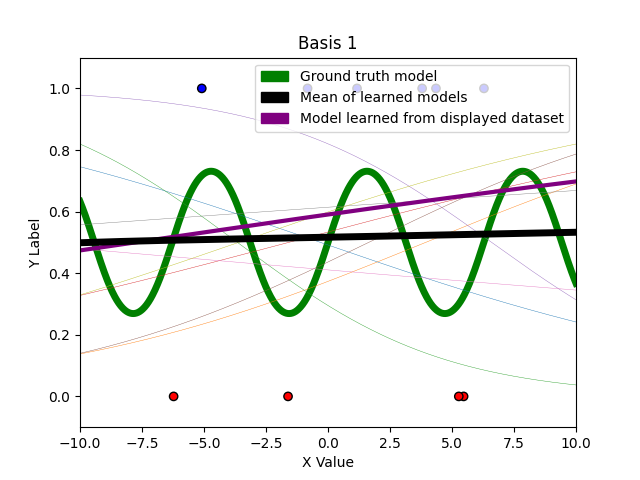
\includegraphics[width=.7\textwidth]{Basis 1.png}

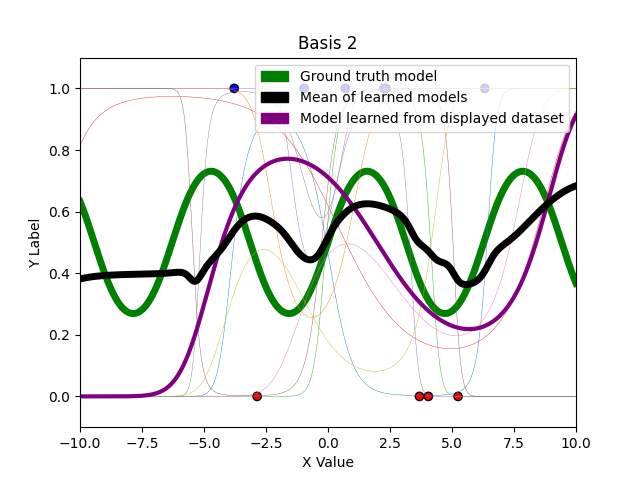
\includegraphics[width=.7\textwidth]{Basis 2.png}

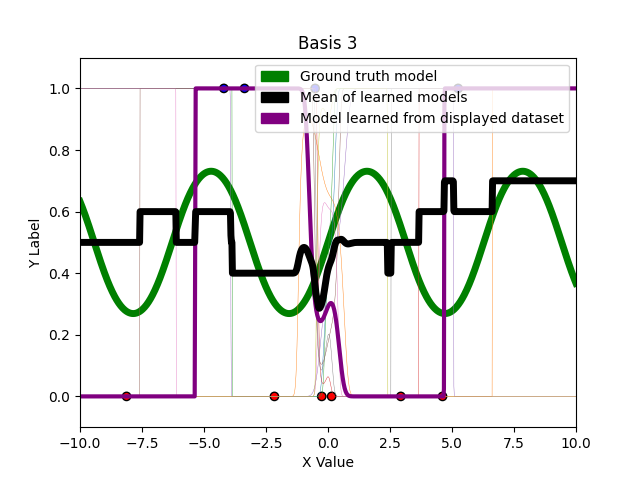
\includegraphics[width=.7\textwidth]{Basis 3.png}

    \item We can observe the effects of the bias-variance trade-off from this visuals. Basis 1's model results in high bias and low variance, as we can see both from the individual and mean of learned models.  Basis 3's model results in high variance and low bias, as we can see that the data is overfit, while Basis 1's model is underfit. Basis 2 offers a balancing compromise, though variance for the individual models is still quite high. The effects of the high variance in individual models is reduced by taking a mean of the learned models, which exhibits a good balance between bias and variance. The basis, as it increases in number of parameters, is able to capture more exactly a particular dataset by drawing from increasingly large groups of function classes (with Basis 3 encompassing the most options). This results in, as the basis parameters increase, a closer fit per dataset. However, with too many parameters and too many function classes considered, overfitting occcurs, where the model threads through each data point exactly, but doesn't capture the true relationship/generating function very well, especially with a smaller dataset size. 
    
    \item Increasing the dataset for Basis 1 will not have a huge effect, since the bias will likely remain high due to the basis itself being an non-optimal (introduces a bias that is not similar to the true distribution). However, for Basis 2 and 3, additional data will reduce variance and lead to fits, especially the mean of learned models, that are closer to the true generating model. This will be especially true for Basis 2, since for Basis 3, the learned models might have lower variance since they will thread through more data points, which will hopefully be spread evenly such that we have fewer big jumps in the y-label across the x-values. However, with Basis 3, we might still see that the data is overfit unless we significantly increase the dataset size. I experimented with increasing to N=60, but still saw a lot of variance with Basis 3. Here are all my visuals for each basis, but for N=60, illustrating what I've just discussed in comparison to N=10. 
    
    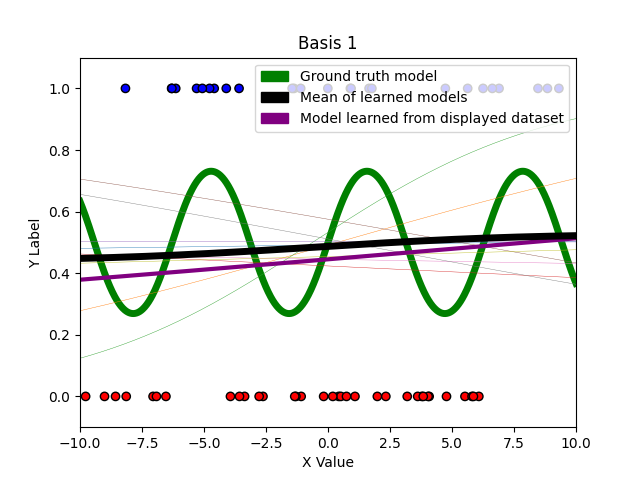
\includegraphics[width=.7\textwidth]{Basis1-60pts.png}

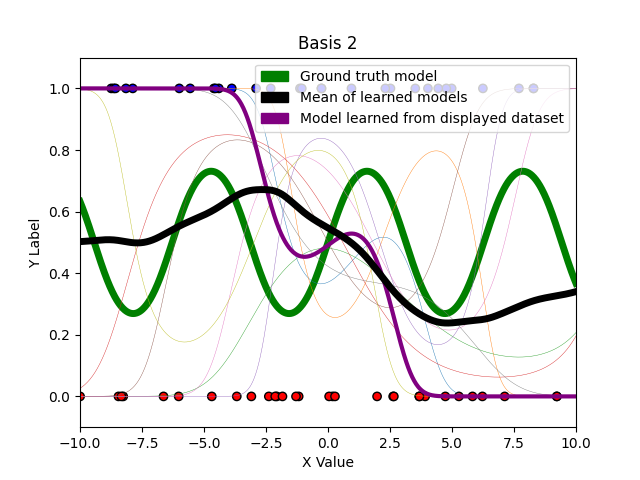
\includegraphics[width=.7\textwidth]{Basis2-60pts.png}

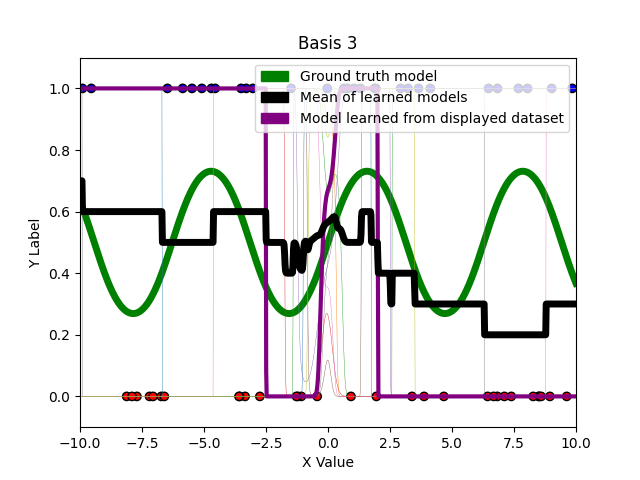
\includegraphics[width=.7\textwidth]{Basis3-60pts.png}
\end{enumerate}

%%%%%%%%%%%%%%%%%%%%%%%%%%%%%%%%%%%%%%%%%%%%%
% Problem 2
%%%%%%%%%%%%%%%%%%%%%%%%%%%%%%%%%%%%%%%%%%%%%
\begin{problem}[Maximum likelihood in classification, 15pts]

  Consider now a generative $K$-class model.  We adopt class prior
  $p(\boldy = C_k; \bpi) = \pi_k$ for all $k \in \{1, \ldots, K\}$
(where $\pi_k$ is a parameter of the prior).
Let  $p(\boldx|\boldy=C_k)$ denote
the class-conditional density of features $\boldx$ (in this
case for class $C_k$). Consider the data set $D = \{(\boldx_i,
\boldy_i)\}_{i=1}^n$ where as above $\boldy_i \in \{C_k\}_{k=1}^K$ is
encoded as a one-hot target vector and the data are independent.

\begin{enumerate}
  \item Write out the negative log-likelihood of the data set, $-\ln p(D ; \bpi)$.

  \item Since the prior forms a distribution, it has the constraint that
    $\sum_k\pi_k - 1 = 0$.  Using the hint on
Lagrange multipliers below, give the
    expression for the maximum-likelihood estimator for the prior
    class-membership probabilities, i.e.
    $\hat \pi_k.$
    Make sure to write out the intermediary equation you need
    to solve to obtain this estimator. Briefly state why your final answer is intuitive.
\end{enumerate}

    For the remaining questions, let the
    class-conditional probabilities be Gaussian distributions with
the same covariance matrix
    $$p(\boldx | \boldy = C_k) = \mathcal{N}(\boldx |  \bmu_k, \bSigma), \text{\ for\ }k \in \{1,\ldots, K\}$$
    and different means $\bmu_k$ for each class.

    \begin{enumerate}
  \item[3.] Derive the gradient of the negative log-likelihood with respect to vector $\bmu_k$.
    Write the expression in matrix form as a function of the variables defined
    throughout this exercise. Simplify as much as possible for full credit.
  \item[4.] Derive the maximum-likelihood estimator $\hat{\mu}_k$ for vector $\bmu_k$. Briefly state why your final answer is intuitive.
  \item[5.] Derive the gradient for the negative log-likelihood with respect to the
    covariance matrix $\bSigma$ (i.e., looking
to find an MLE for the covariance).
Since you are differentiating with respect to a
    \emph{matrix}, the resulting expression should be a matrix!
%
  \item[6.] Derive the maximum likelihood estimator $\hat{\Sigma}$ of the covariance matrix.
\end{enumerate}

\paragraph{Hint: Lagrange Multipliers.} Lagrange Multipliers are a method for
optimizing a function $f$ with respect to an
equality constraint, i.e.
\[\min_{\boldx} f(\boldx)\ \text{s.t.}\ g(\boldx) = 0.\]

This can be turned into an unconstrained problem by introducing a
Lagrange multiplier $\lambda$ and constructing the Lagrangian function,
\[L(\boldx, \lambda) =  f(\boldx) + \lambda g(\boldx).\]

It can be shown that it is a necessary condition that the optimum
is a critical point of this new function. We can find this point by solving two equations:

\[\frac{\partial L(\boldx, \lambda)}{\partial  \boldx} = 0  \ \ \text{and}\  \  \frac{\partial L(\boldx, \lambda)}{\partial \lambda} = 0 \]


\paragraph{Cookbook formulas.} Here are some formulas you might want to consider
using to compute difficult gradients. You can use them  in the homework
without proof. If you are looking to hone your matrix calculus skills, try to
find different ways to prove these formulas yourself (will not be part of the
evaluation of this homework). In general, you can use any formula from the matrix cookbook,
as long as you cite it. We opt for the following common notation:
$\boldX^{-\top} := (\boldX^{\top})^{-1}$
\begin{align*}
  & \frac{\partial \bolda^\top \boldX^{-1} \boldb}{\partial \boldX} = - \boldX^{-\top} \bolda \boldb^\top \boldX^{-\top} \\
  & \frac{\partial \ln | \det (\boldX) |}{\partial \boldX} = \boldX^{-\top}
 \end{align*}
 \end{problem}


\subsection*{Solution}

\begin{enumerate}
    \item Using the product rule for logs multiple times, we get the following, as already shown partially in section:
    
    $\mathcal{L} = -\ln p(D; \boldsymbol{\pi}) = -\sum_{i=1}^n \ln p(\boldsymbol{x_i}, \boldsymbol{y_i}|\boldsymbol{\pi}) = -\sum_{i=1}^n (\ln p(\boldsymbol{x_i}|\boldsymbol{y_i}, \boldsymbol{\pi}) + \ln p(\boldsymbol{y_i}|\boldsymbol{\pi})) $
    
    $= -\sum_{i=1}^n [\sum_{j=1}^K y_{ij}(\ln p(\boldsymbol{x_i}|\boldsymbol{y_i} = C_j, \boldsymbol{\pi}) + \ln \pi_j)]$
    
    \item We can construct our Lagrange function as follows to incorporate the given constraint:
    
    $\mathcal{L(\boldsymbol{\pi}, \lambda)} = -\sum_{i=1}^n [\sum_{j=1}^K y_{ij}(\ln p(\boldsymbol{x_i}|\boldsymbol{y_i} = C_j, \boldsymbol{\pi}) + \ln \pi_j)] + \lambda((\sum_{j=1}^K \pi_j) - 1)$
    
    We take the two derivatives of this function with respect to our prior and lambda, and set them to zero to get the following:
    
    $\pdv{\mathcal{L}}{\pi_j} = \sum_{i=1}^N \frac{y_{ij}}{\pi_j} - \lambda = 0$
    
    $\frac{1}{\pi_j} \sum_{i=1}^N y_{ij} = -\lambda$
    
    $\pi_j = -\frac{1}{\lambda} \sum_{i=1}^N y_{ij}$
    
    $\pdv{\mathcal{L}}{\lambda} = (\sum_{j=1}^K \pi_j) - 1 = 0$
    
    $(\sum_{j=1}^K \pi_j) = 1$
    
    Substituting in from earlier, we get:
    
    $\sum_{i=1}^N[\sum_{j=1}^K -\frac{1}{\lambda} y_{ij}] = 1$
    
     $-\frac{1}{\lambda}\sum_{i=1}^N\sum_{j=1}^K  y_{ij} = 1$
     
     $-\frac{1}{\lambda}\sum_{i=1}^N 1 = 1$
     
     $-\frac{1}{\lambda}N = 1$
     
     $\lambda = -N$
     
     Substituting again, we get:
     
     $\hat{\pi}_j = \frac{1}{N} \sum_{i=1}^N y_{ij}$
     
     This result is intuitive since if we were to empirically estimate the probability that a certain class occurs, we would look to our dataset and count the number of times that class appears and divide by the size of our dataset. This is what the above expression captures.
     
     \item We can borrow some section results surrounding applying the log to the Gaussian pdf for the conditional probability portion of our loss to see that we will be taking the gradient of:
     
     $\sum_{i=1}^N y_{ik}[-\frac{1}{2}\ln |\boldsymbol{\Sigma}| - \frac{1}{2}(\boldsymbol{x_i} - \boldsymbol{\mu_k})^T \boldsymbol{\Sigma}^{-1}(\boldsymbol{x_i} - \boldsymbol{\mu_k})]$
     
     Note that $y_{ik}$ is derived from the on-hot encoding and is equal to 1 if the $i$th data point is in class $k$, otherwise, this is equal to 0. Taking the gradient (of this truncated portion of the loss that involves the $\boldsymbol{\mu_k}$ term, which is what we care about here) with respect to $\mu_k$ gives us:
     
     $\frac{1}{2}\sum_{i=1}^N y_{ik} \boldsymbol{\Sigma}^{-1}(\boldsymbol{x_i} - \boldsymbol{\mu_k})$
     
     \item We set the gradient from the previous part equal to zero to get the following:
     
     $\frac{1}{2}\sum_{i=1}^N y_{ik} \boldsymbol{\Sigma}^{-1}(\boldsymbol{x_i} - \boldsymbol{\mu_k}) = 0$
     
     $\sum_{i=1}^N y_{ik} \boldsymbol{\Sigma}^{-1}\boldsymbol{x_i}  = \sum_{i=1}^N y_{ik} \boldsymbol{\Sigma}^{-1} \boldsymbol{\mu_k}$
     
     If we left multiply both sides by $\boldsymbol{\Sigma}$, we can then use the commutative property to left multiply it directly against the $\boldsymbol{\Sigma}^{-1}$ to get the identity matrix and essentially remove $\boldsymbol{\Sigma}$ from both sides we get
     
     $\sum_{i=1}^N y_{ik} \boldsymbol{x_i}  = \sum_{i=1}^N y_{ik} \boldsymbol{\mu_k}$
     
     Then, rearranging to solve for $\mu_k$ gives us:
     
     $\hat{\mu}_k = \frac{\sum_{i=1}^N y_{ik} \boldsymbol{x_i}}{\sum_{i=1}^N y_{ik} }$
     
     This answer is intuitive because if we were to get the mean of our x's for a certain class, we would only consider the data points of that class, sum the x's up, and divide by the number of data points we have in that class. This would essentially take the average of the x vectors from that class, which is what our expression captures. 
     
     \item  Again, we can borrow some section results surrounding applying the log to the Gaussian pdf for the conditional probability portion of our loss to see that we will be taking the gradient of:
     
     $\sum_{i=1}^N \sum_{j=1}^K y_{ij}[-\frac{1}{2}\ln |\boldsymbol{\Sigma}| - \frac{1}{2}(\boldsymbol{x_i} - \boldsymbol{\mu_j})^T \boldsymbol{\Sigma}^{-1}(\boldsymbol{x_i} - \boldsymbol{\mu_j})]$
     
     Note that unlike for Part 3, we still need to keep the $\sum_{j=1}^K$ portion of this expression because $\boldsymbol{\Sigma}$ is a part of each term of this sum, whereas $\mu_k$ was only part of the term of the sum for its associated $j=k$. 
     
     Taking the derivative of this expression (truncated portion of the loss that involves the $\boldsymbol{\Sigma}$ term) and using the matrix cookbook formulas, we get:
     
     $\sum_{i=1}^N\sum_{j=1}^K[-\frac{1}{2}\boldsymbol{\Sigma}^{-T} + \frac{1}{2}\boldsymbol{\Sigma}^{-T}(\boldsymbol{x_i} - \boldsymbol{\mu_j}) (\boldsymbol{x_i} - \boldsymbol{\mu_j})^T\boldsymbol{\Sigma}^{-T}]$.
     
     \item Setting the above gradient equal to zero, we have that:
     
     $\sum_{i=1}^N\sum_{j=1}^K[-\frac{1}{2}\boldsymbol{\Sigma}^{-T} + \frac{1}{2}\boldsymbol{\Sigma}^{-T}(\boldsymbol{x_i} - \boldsymbol{\mu_j}) (\boldsymbol{x_i} - \boldsymbol{\mu_j})^T\boldsymbol{\Sigma}^{-T}] = 0$
     
     Using a similar operation as seen before, we can right and left multiply each term in this sum and rearrange the result around the equal sign to get:
     
     $\sum_{i=1}^N\sum_{j=1}^K y_{ij}\boldsymbol{\Sigma}^T = \sum_{i=1}^N\sum_{j=1}^K y_{ij}(\boldsymbol{x_i} - \boldsymbol{\mu_j}) (\boldsymbol{x_i} - \boldsymbol{\mu_j})$.
     
     Then solving for $\boldsymbol{\Sigma} = \boldsymbol{\Sigma}^T$ gives us the following, where we can use the fact that $\boldsymbol{\Sigma}$ is symmetric (meaning $\boldsymbol{\Sigma} = \boldsymbol{\Sigma}^T$):
     
     $\boldsymbol{\Sigma} = \frac{\sum_{i=1}^N\sum_{j=1}^K y_{ij}(\boldsymbol{x_i} - \boldsymbol{\mu_j}) (\boldsymbol{x_i} - \boldsymbol{\mu_j})}{\sum_{i=1}^N\sum_{j=1}^K y_{ij}}$
     
\end{enumerate}

%%%%%%%%%%%%%%%%%%%%%%%%%%%%%%%%%%%%%%%%%%%%%
% Problem 3
%%%%%%%%%%%%%%%%%%%%%%%%%%%%%%%%%%%%%%%%%%%%%

\begin{problem}[Classifying Stars, 15pts]

You're tasked with classifying three different kinds of stars using their magnitudes and temperatures. See star.png for a plot of
the data, adapted from
\url{http://astrosci.scimuze.com/stellar_data.htm} and available as
\verb|data/hr.csv|, which you will find in the Github repository. \\

The CSV file has three columns: type, magnitude, and temperature. The
first few lines look like this:
\begin{csv}
Type,Magnitude,Temperature
Dwarf,-5.8,-0.35
Dwarf,-4.1,-0.31
...
\end{csv}

In this problem, you will code up 4 different classifiers for this task:
\begin{enumerate}[label=\alph*)]

\item \textbf{A three-class generalization of logistic regression}, also
  known as softmax regression, in which you implement gradient descent on the negative log-likelihood. In Question 2 you will explore the effect of using different values for the learning rate $\eta$ (\texttt{self.eta}) and
  regularization strength $\lambda$ (\texttt{self.lam}).  Make sure to include a bias term and to
  use L2 regularization. See CS181 Textbook's Chapter 3.6 for details on multi-class
  logistic regression and softmax.
  
\item \textbf{A generative classifier with Gaussian class-conditional
  densities with a \textit{shared covariance} matrix} across all classes. 
  Feel free to re-use your Problem 2 results.
\item \textbf{Another generative classifier with Gaussian class-conditional densities , but now 
with a \textit{separate covariance} matrix} learned for each class. (Note: 
The staff implementation can switch between the two Gaussian generative classifiers with just a
few lines of code.)

\item \textbf{A kNN classifier} in which you classify based on the $k=1,3,5$ nearest neighbors and the following distance function: $$dist(star_1, star_2) = ((mag_1 - mag_2)/3)^2 + (temp_1 - temp_2)^2$$
where nearest neighbors are those with the smallest distances from a given point.

  Note 1: When there are more than two labels, no label may have the
  majority of neighbors.  Use the label that has the most votes among
  the neighbors as the choice of label. 

  Note 2: The grid of points for which you are making predictions
  should be interpreted as our test space.  Thus, it is not necessary
  to make a test point that happens to be on top of a training point
  ignore itself when selecting neighbors.

\end{enumerate}

After implementing the above classifiers, complete the following exercises:

\begin{enumerate}
    \item Plot the decision boundaries generated by each classifier for the dataset. Include them in your PDF. 
    Identify the similarities and differences among the classifiers. What explains the differences?
    
    \item For logistic regression only,  make a plot with
      ``Number of Iterations" on the x-axis and ``Negative Log-Likelihood Loss" on the y-axis for several
      configurations of the hyperparameters $\eta$ and $\lambda$.  Specifically,  try the values $0.05$,  $0.01$,  and $0.001$ for each hyperparameter.  Limit the number of gradient descent iterations to 200,000.  What are your final choices of learning rate
      ($\eta$) and regularization strength ($\lambda$), and why are they reasonable? How
      does altering these hyperparameters affect the ability to converge,  the rate of convergence,  and the final loss (a qualitative description is sufficient)? You only need to submit one plot for your final choices of hyperparameters.

    \item For both Gaussian generative models, report the negative log-likelihood loss. Which model has a lower loss, and why?
      For the separate covariance model, be sure to use
      the covariance matrix that matches the true class of each data
      point.
    
    \item Consider a star with Magnitude 6 and Temperature 2.
      To what class does each classifier assign this star? Do the
      classifiers give any indication as to whether or not you should
  trust them?
\end{enumerate}
\end{problem}

\newpage

\begin{framed}
\noindent\textbf{Problem 3} (cont.)\\


\textbf{Implementation notes:} Run the controller file, \texttt{T2\_P3.py},
to test your code. Write the actual implementations in the \texttt{GaussianGenerativeModel},
\texttt{LogisticRegression}, and \texttt{KNNModel} classes, which are defined in the three
\texttt{T2\_P3\_ModelName.py} files. These classes follow the same interface pattern
as sklearn. Their code
currently outputs nonsense predictions just to show the
high-level interface, so you should replace their \texttt{predict()} implementations.
You'll also need to modify the hyperparameter
values in \texttt{T2\_P3.py} for logistic regression.
\end{framed}

\newpage

\subsection*{Solution}

\begin{enumerate}
    \item Plots:
    
    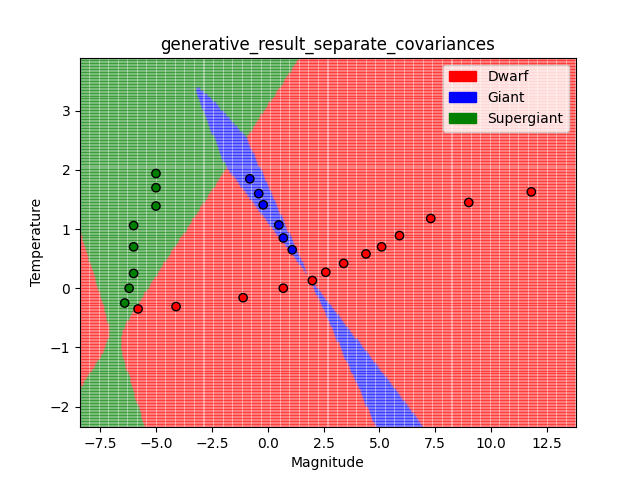
\includegraphics[width=.7\textwidth]{generative_result_separate_covariances.png}
    
    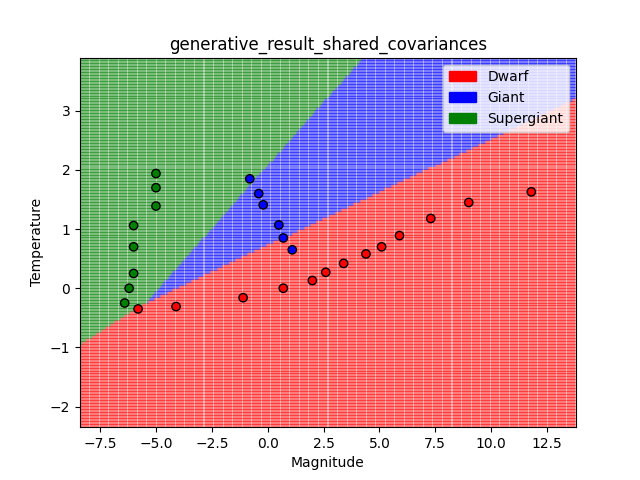
\includegraphics[width=.7\textwidth]{generative_result_shared_covariances.png}
    
    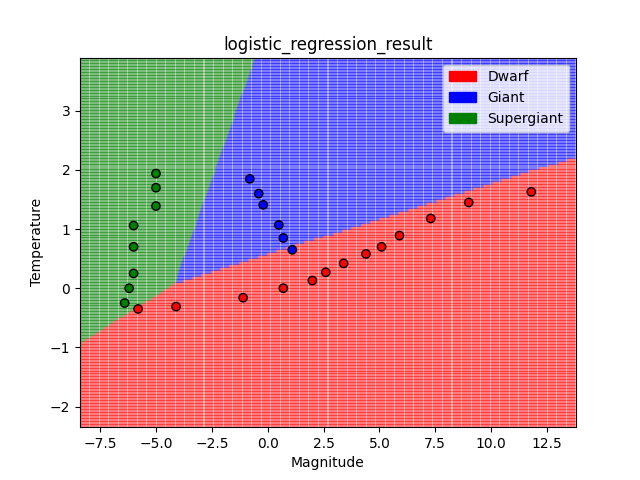
\includegraphics[width=.7\textwidth]{logistic_regression_result.png}
    
    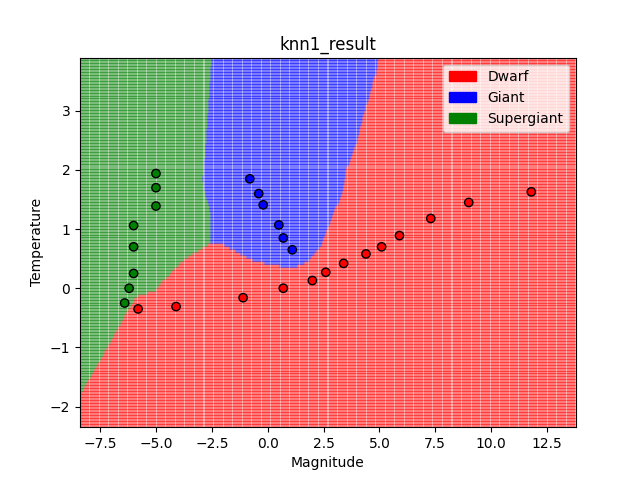
\includegraphics[width=.7\textwidth]{knn1_result.png}
    
    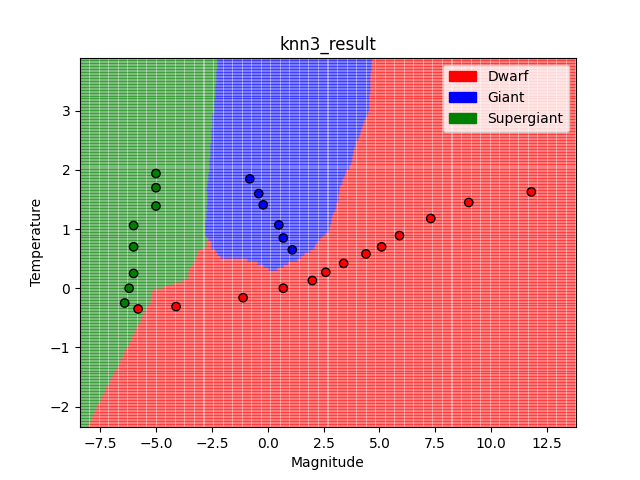
\includegraphics[width=.7\textwidth]{knn3_result.png}
    
    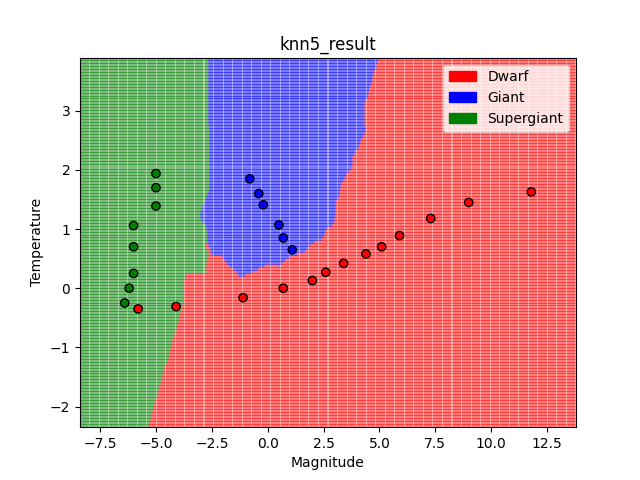
\includegraphics[width=.7\textwidth]{knn5_result.png}
    
    The KNN plots all look distinctive from the other classifiers. With k=1, each predicted point takes the label from the "closest" data point, and as we increase k up to k=5, we end up taking the majority class (breaking ties arbitrarily using python's functionality) of the nearest 5 neighbors, which produces some perturbations in the boundaries between classes, especially since there are regions where, for example, green and red points are in close proximity. In those areas, there are, density-wise, more green points, leading the green portion to encroach on the red portion (bottom left). We can see something similar near the center of the plot as the red region encroaches on the blue region. 
    
    The Gaussian with separate covariances also looks uniquely distinctive, though it almost makes the most intuitive sense. This is because it is reasonable to assume, even beyond the x-data we have, that the different types of stars have distinctive qualities and stars of each type might vary against each other in a way that is distinct from the way other types vary against each other. Therefore, it is quite reasonable to think that the different star types are best classified with separate covariances, and the blue giant's region is able to carve out a distinctive sliver of area out of the red region because of the particular way that data varies in contrast to the way the dwarfs might. We don't see this type of "cut" of the blue region across the red region in any other plot. 
    
    The generative result with shared covariance looks quite similar to the logistic regression result. This is at least partially because, similar to the logistic regression, the boundaries of generative classification with shared covariance has linear boundaries, whereas generative with separate covariance has quadratic boundaries, enabling the aforementioned "cut" of the blue region. Since the logistic regression might be able to better penalize misclassified points over time and push boundaries a certain way to eliminate all outliers from misclassification, the logistic regression shows fewer misclassifed points whereas the generative with shared covariance doesn't penalize this as strictly but instead focuses on finding parameters that created distributions that best fit observed data.
    
    \item My final choice was a learning rate of 0.05 and a regularization strength of 0.001. This was motivated by the following loss results:
    
    \begin{center}
        \begin{tabular}{ |c|c|c|c| } 
         \hline
         \eta / \lambda & $\lambda = 0.001$ & $\lambda = 0.01$ & $\lambda = 0.05$ \\
         \hline
         $\eta = 0.001$ & 4.273 & 6.929 & 11.412\\ 
         \hline
         $\eta = 0.01$ & 2.835 & 6.882 & 11.412\\ 
         \hline
         $\eta = 0.05$ & 2.829 & 6.882 & 11.412\\ 
         \hline
        \end{tabular}
    \end{center}
    
    Overall, a lower learning rate led to lower speed of convergence, since the size of each update was relatively small, requiring more steps to achieve the same loss. Thus, the graphs of loss over time for lower learning rate had a more gradual slope, compared to higher learning rate, which had a much steeper fall in the loss over just a few steps. However, there were instances where if learning rate was set of 0.05, perhaps too high, the loss would oscillate around a value rather than continuing to decrease over time. Thus, a higher learning rate might affect the ability to converge, since the updates might cause the loss to jump back and forth around the true minimum, but never actually reach it. 
    
    The regularization strength essentially limits the magnitude of the elements of W. For this model, it seemed that stronger regularization resulted in slightly higher loss. This signals to us that regularization is not desired for this model and that we do want our terms of W to be freer to take more extreme values. There are perhaps cases where regularization can speed up rate of convergence, such as when the objective function is more oblong; in this case, regularization can make it more bowl-shaped and speed up convergence. However, regularization could also distract us from optimizing our "true" objective function and lead to slower convergence or even hinder our ability to truly achieve zero loss on our objective due to the addition of a regularization term/bias. This latter case seems to be what we observe for this model, with the regularization strength controlling our ability to convergence more than the learning rate it seems.
    
    Here is my plot for my final choice of these parameters:
    
    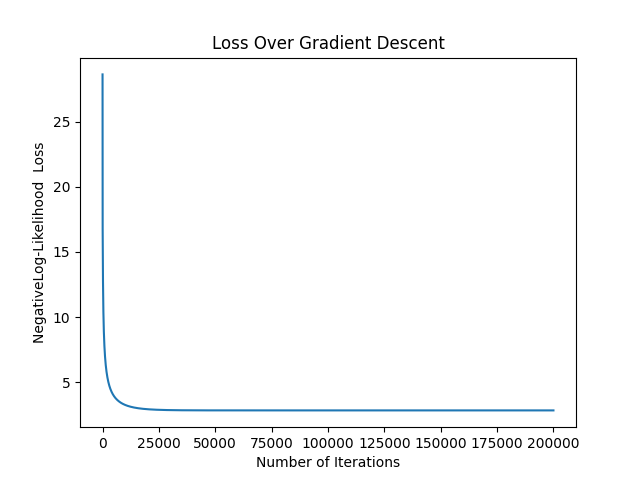
\includegraphics[width=.7\textwidth]{LogRegLoss.png}
    
    \item The generative with separate covariances has a loss of 63.9703598409242 and the generative with shared covariance has a loss of 116.39446507788162. Thus, the Gaussian with separate covariances has the lower loss, and this is because since the types of stars exhibited each their unique pattern of data, with the data points for each type varying in a unique way compared to data points for other star types, the separate covariances was able to capture this unique variation for each type and factor that into maximizing likelihood, which overall resulted in fewer giants (blue) being misclassfied. This intuitively makes sense, since with the current data trends, we would expect the giants data to trend down and to the right, perhaps cutting across the red region. Separate covariance thus is best able to capture the differences between different star types (which are likely data best generated from unique distributions that take into account the unique features of each star type), and thus makes realistically and intuitively the most sense. 
    
    \item We get the following predicted classifications:
    
    \begin{itemize}
        \item Test star type predictions for Separate Covariance Gaussian Model: magnitude 6 and temperature 2: 0
        \item Test star type predictions for Shared Covariance Gaussian Model:
        magnitude 6 and temperature 2: 1
        \item Test star type predictions for Linear Regression: magnitude 6 and temperature 2: 1
        \item Test star type predictions for KNN Model with k=1:
        magnitude 6 and temperature 2: 0
        \item Test star type predictions for KNN Model with k=3:
        magnitude 6 and temperature 2: 0
        \item Test star type predictions for KNN Model with k=5:
        magnitude 6 and temperature 2: 0
    \end{itemize}

    For previously mentioned reasons, the generative with separate covariance is likely the most trustworthy, but we would need more data to confirm the trends in each type of star. For the generative with shared covariance and logistic regression, which look quite similar as mentioned previously, it seems perhaps dubious that stars with both high magnitude and high temperature are all giants, where as those with high magnitude and low temperature are all dwarfs. These are regions where we have relatively little data, but if we were to perhaps fit trend lines individually to each star type, we might expect a result similar to the generative with separate covariance. Further data, again, would be necessary to confirm these results. With near identical justification, the predictions for the KNN are also dubious. This is especially true for KNN's since with little data, we are not able to make the best fine-grained predictions, especially for inputs that are "far" from all available data points. Therefore, we see huge swaths of the plot classified as dwarf, which might not be the truth. 
    
    It is also notable that despite the generative with separate covariance giving an "intuitive" result, it's NLL loss was still much higher than the logistic regression, which has been optimized to minimize this loss. The same can be seen when comparing the generative with shared covariance and logistic regression. That's not to say the boundaries are all that poorly made, but it is something to consider. 
    
    
\end{enumerate}

\newpage
%%%%%%%%%%%%%%%%%%%%%%%%%%%%%%%%%%%%%%%%%%%%%
% Name and Calibration
%%%%%%%%%%%%%%%%%%%%%%%%%%%%%%%%%%%%%%%%%%%%%
\subsection*{Name}

Kathryn Wantlin

\subsection*{Collaborators and Resources}
Whom did you work with, and did you use any resources beyond cs181-textbook and your notes?

Nari, Andrew, Ryan, Sanjana, Mark, Yash's OH. Also collaborated with Justine Boudou and used section results.

\subsection*{Calibration}
Approximately how long did this homework take you to complete (in hours)?

15 hrs

\end{document}
